\section{Skin recognition}
    Liveness detection motivations.

    Fast face detection motivations.

    \subsection{How it works?}
        Wide description about material detection
        with light reflectiveness.

    \subsection{Technical aspect -- how camera works?}
        To think about security aspect of skin detection,
        it's critical to understand how image sensors works.
        Most common are \textit{CCD} (\textit{charge-coupled device})
        and \textit{CMOS} (\textit{complementary metal-oxide-semiconductor})
        [TODO: LINK NEEDED]. % Most common?
        Due to better quality, as well as sensitiveness, for security reasons
        it probably would be better to use CCD.
        However, both matrices have same problem -- limitation on wavelength sensitivity.
        Such sensors are sensitive to wavelengths aproximetly up to 1050nm,
        which may be serious limitation as skin ligthen with greater wavelength has
        more undifferentiated characteristics.
        Therefore looking for best possible skin detection method,
        it may be convenient to assume that other type of light sensitive matrices
        are in reach of inventor.
        Nevertheless we were limited to very common cameras.

        TODO: Paragraph about light sensors materials and other types of image sensors.
        Paragraph under maintenance. May dissapear.

        We are describeing one possible realization, keep in mind that
        there are more solutions than that, but we don't find them usfeful in our problem.

        \subsubsection*{Monochrome}
            As image sensor is matrix build from many small photodiodes,
            % TODO: in fact working like...
            it's natural to create monochromatic image.
            Because photodiodes don't distinguish different
            wavelength, only light intensity, it's hard
            to measure light reflectiveness.
            The only possible way to do that is to
            make different picture for every wavelength.
            It's not easy, as you have to
            provide your own lighting and somehow remove
            light coming from other sources.
            Also, all pictures have to be made in
            a~very short time interval, as the subject
            cannot move between shots.

        \subsubsection*{Multispectral imaging}
            Multispectral imaging is answer to
            problem of object's move,
            way to measure every wavelength intensity in one picture.
            Probably easies way to describe it is to look at RGB camera.
            There every photodiode is responsible for exacly one colour,
            where as colour we understand wavelength interval (it's important
            to understand, that we can consider any wavelength interval as one colour).
            And result picture is built from small squares (mostly $2 \times 2$)
            of photodiode matrix data.
            There may be more than just  three colours in fact.
            For example, you may find camera which see two types of ''green''.
            Mostly, at the end everything is converted to known RGB format.

            \begin{center}
                \includegraphics{RGB-matrix}
            \end{center}

            Software receives from camera imformation with light intensity at every
            sensor and information which colour it sees. 

            One from possible realisations of reducing the range
            of light visible through the sensor is to take standard image sensor which
            may see full specturm of light ($350$-$1050$nm.) and
            place filters in way that only specific light will reach choosen photodiode.

            \begin{center}
                \includegraphics[scale=0.40]{RGB-filter}
            \end{center}

        \subsubsection*{Hyperspectral imaging}
            Hyperspectral imaging is creating pictures using camera with
            capabilityy to distinguish many and many of colours (more like hundreds or thousands)
            insted of just few.
            It would be very helpful, obviously, in skin-detection device,
            but there is very little chance to see such device in mobile phones soon.

    \subsection{Technical aspect -- how it may be created?}
        As we know how camera works, we can say that there are only two ways of
        building skin detection mobile device.
        \subsubsection*{Monochrome}
            We can work without filters (or with one for whole camera),
            but then we have to make picture for every wave lenght.
            Also, we need one diode with that very wavelength we want.
            It's easier method to build in phone, but taking pictures
            must be very fast.

            Bigest pros of that solution is possibility of lighting
            with different LEDs in random moment of time, so hackers
            will no be able to play with own diods to modify result.

        \subsubsection*{Multispectral imaging}
            Also there is possibility to use filters with specific infrared colours.
            But important here is avoiding standard smoothing algorithms used
            in cameras. We truly need real light intensity from every sensor.
            Not smoothed or reduced one.

    \subsection{Results}
        Wide discussion about results.

        \subsubsection*{Prototype}
            ...

    \subsection{RGB skin detection symulation}
        Using RGB to deteckt skin on picture.
        Mtoivations.

        Description of not ours solutions.

        \subsubsection*{Case-study}
            Description of problem using math.
            Final algorithm.
